\subsection{Rete neurale con elementi di ritardo}

Una rete neurale con elementi di ritardo presenta un uscita dipendente, oltre che dagli ingressi attuali e dagli stati della rete, anche dagli ingressi passati (ottenuti tramite ritardi o delays) ed uscite passate (ottenute tramite feedbacks).

Scopo di queste reti è quello di usare valori passati di una serie temporale per predire quelli futuri: se indichiamo con x(t) il vettore di input all’istante t, e con y(t) il vettore di output al medesimo istante, abbiamo che y(t) sarà funzione degli ultimi N vettori risultato del sistema e degli ultimi N vettori di input.

%% FIXME: riscrivere usando sintassi latex standard
%% $$
%% y(t)=f(y(t\lyxmathsym{\textminus}1),y(t\lyxmathsym{\textminus}2),...,y(t\lyxmathsym{\textminus}N),x(t\lyxmathsym{\textminus}1),x(t\lyxmathsym{\textminus}2),...,x(t\lyxmathsym{\textminus}N))
%% $$

Anche in questo caso, ad ogni passo dell'addestramento, il vettore di output generato dal sistema viene confrontato con il corrispondente vettore obiettivo, e a seconda della differenza vengono opportunamente aggiornati i pesi dei neuroni che compongono gli strati nascosti e lo strato di uscita, fino ad ottenere un livello di generalizzazione soddisfacente.

L'approccio usato per la modellizzazione di questa rete è del tutto analogo a quello usato con la rete neurale statica prima enunciata, l'unica differenza è che questa volta, per agevolare ulteriormente l'apprendimento della rete neurale, è stato decisio di creare una rete per ogni tipo di uscita; sono quindi state modellizzate due reti distinte: una per l'energia stimata ed una per la luminosità interna all'edificio.

Infine anche in questo caso poteva essere utilizzato direttamente il tool proposto da Matlab (nntstool), usufruendo quindi della GUI proposta, ma per gli stessi inconvenienti già esposti, è stato deciso di creare uno script analogo al caso precedente per ricavare questo tipo di rete in modo automatico.

Il tipo di rete che tratteremo in questa sezione è quella mostrata nella figura seguente:

\begin{figure}[htbp]
  \centering
  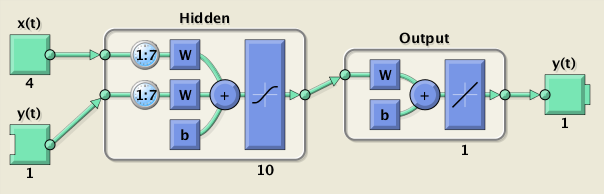
\includegraphics[scale=0.5]{images/timeseries/energia/net.png}
  \caption{Rete neurale esogena autoregressiva}
\end{figure}


\subsubsection{Suddivisione dei dati}

Il primo passo per la creazione delle due reti è stato quello di suddividere i dati riportati nel file csv, creato da conform.rb, in due divesi files, ottenendo dunque un totale di quattro files.

I primi due conterranno gli ingressi delle reti ( i due files sono identici ), i secondi due invece conterranno una diversa colonna di uscita: energia consumata e luminosità interna rispettivamente.


\paragraph{Script energy.rb}

Questo semplice script ruby elabora il file conformData.csv ed estrapola la colonna di uscita inerente all'energia consumata, creando dunque due ulteriori files ( inputEnergy e targetEnergy ) i quali riporteranno al loro interno rispettivamente gli inputs e le relative uscite inerenti all'energia consumata all'interno dello stabile.

\inputminted[linenos=true,fontsize=\footnotesize]{ruby}{../../data/time\ series/energy.rb}
\captionof{listing}{data/time series/energy.rb}


\paragraph{Script inlight.rb}

Lo stesso procedimento è stato eseguito anche per la luminosità interna all'edificio.

\inputminted[linenos=true,fontsize=\footnotesize]{ruby}{../../data/time\ series/inlight.rb}
\captionof{listing}{data/time series/inlight.rb}


\subsubsection{Rircerca della migliore rete neurale}
Nell'ottica di automatizzare il processo di creazione della rete, è stata definita sia una funzione apposita il cui scopo è la ricerca di una rete neurale con elementi di ritardo considerata ottima, sia uno script per la visualizzazione dei risultati ottenuti.

\paragraph{Funzione searchBestTimeSeries}
Scopo di tale funzione è quello di ricercare, se esiste, una rete caratterizzata da parametri ottimali o in alternativa di restituire la rete che ha presentato il miglior apprendimento: quindi con il minor MSE riscontrato ed il più alto coefficiente di regressione.

L'approccio seguito è del tutto simile a quello visto per la modellizzazione di una rete statica; vengono definiti:

\begin{itemize}
  \item Valore minimo e massimo per i delays sia per gli ingressi che per l'uscita.
  \item Numero minimo e massimo di neuroni nascosti
  \item Numero di addestramenti per ogni configurazione di rete
  \item Goals che si desiderano raggiungere, in altre parole le caratteristiche che una rete deve presentare per essere classificata come ottima (in termini di MSE e coefficiente di retta di regressione).
  \item I tre valori cardini di ogni rete neurale: percentuali di test, validation e train.
\end{itemize}

La funzione, partendo dai valori di defaults, modella una rete neurale di tipo esogena auto-regressive (NARX), la allena, la valida ed infine la prova.

Ad ogni passo della funzione vengono fatte variare le variabili sopra enunciate in modo da confrontare tra loro le performances di diverse reti.

Una volta ottenuti i risultati in termini di MSE e retta di regressione ( entrambi inerenti alla fase di test in quanto quella che assicura la generalizzazione ), vengono confrontati con quelli precedentemente salvati e, se migliori, registrati.

Occorre infine dire che anche in questo caso la funzione di addestramento utilizzata è quella standard di backpropagation di Levenberg-Marquardt (trainlm).

\inputminted[linenos=true,fontsize=\footnotesize]{matlab}{../../src/time\ series/functions/searchBestTimeSeries.m}
\captionof{listing}{src/time\ series/functions/searchBestTimeSeries.m}


\paragraph{Script netts.m}
Scopo di questo script matlab è quello di invocare la funzione appena enunciata e di mostrarne i valori restituiti.

\inputminted[linenos=true,fontsize=\footnotesize]{matlab}{../../src/netts.m}
\captionof{listing}{src/netts.m}


\subsubsection{Risultati}

\paragraph{Energia consumata}
%% FIXME: è duplicata!!!
\begin{figure}[htbp]
  \centering
  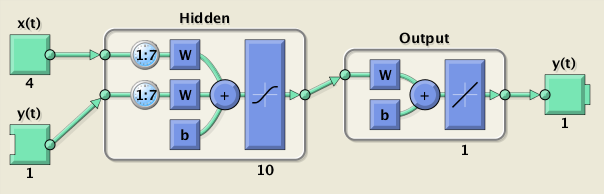
\includegraphics[scale=0.5]{images/timeseries/energia/net.png}
  \caption{Rete usata}
\end{figure}

\begin{figure}[htbp]
  \centering
  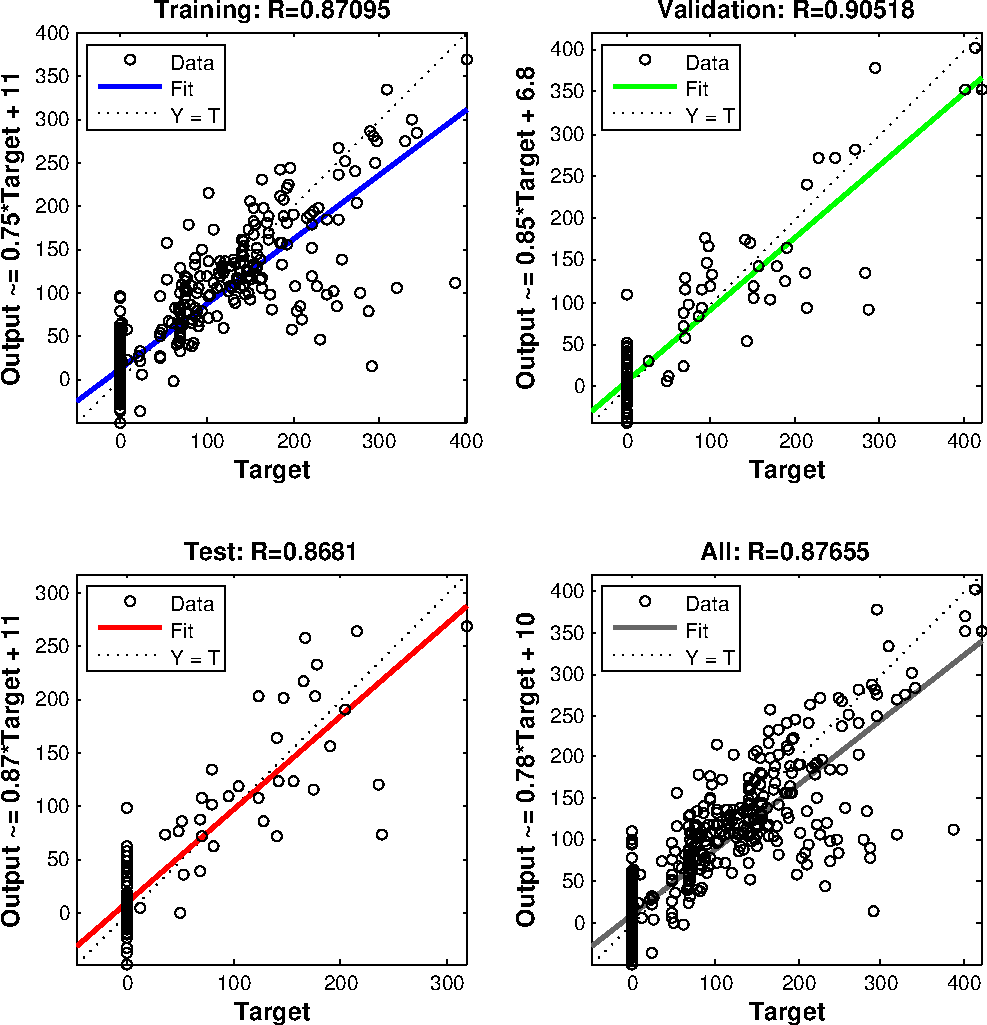
\includegraphics[scale=0.5]{images/timeseries/energia/regressions.pdf}
  \caption{Retta di regressione}
\end{figure}

\begin{figure}[htbp]
  \centering
  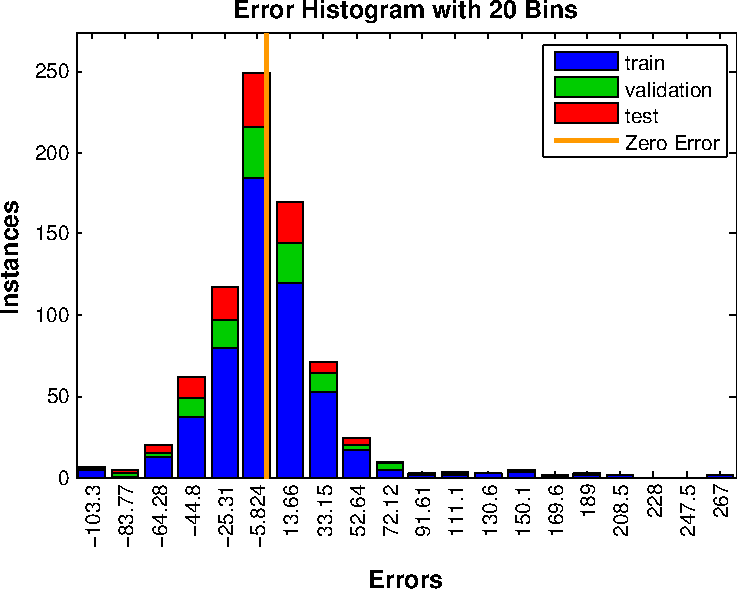
\includegraphics[scale=0.5]{images/timeseries/energia/histogram.pdf}
  \caption{Istrogramma degli errori}
\end{figure}

\begin{figure}[htbp]
  \centering
  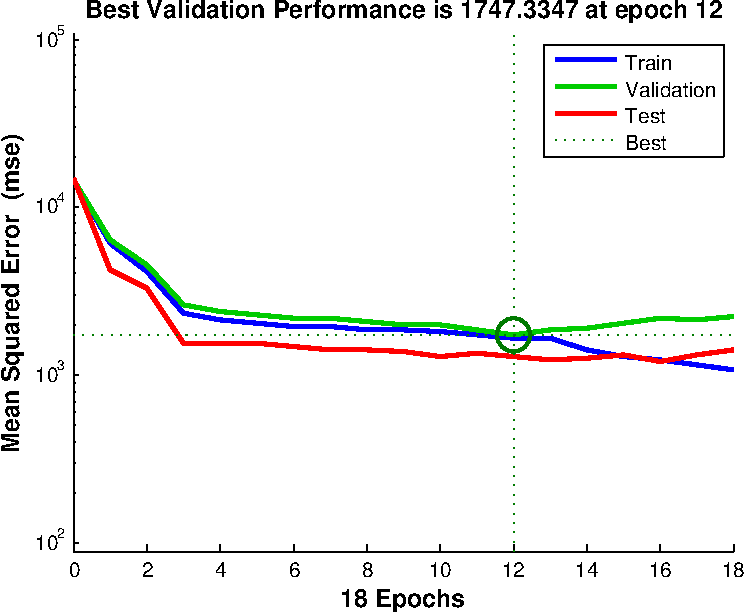
\includegraphics[scale=0.5]{images/timeseries/energia/performances.pdf}
  \caption{Performance}
\end{figure}

\begin{figure}[htbp]
  \centering
  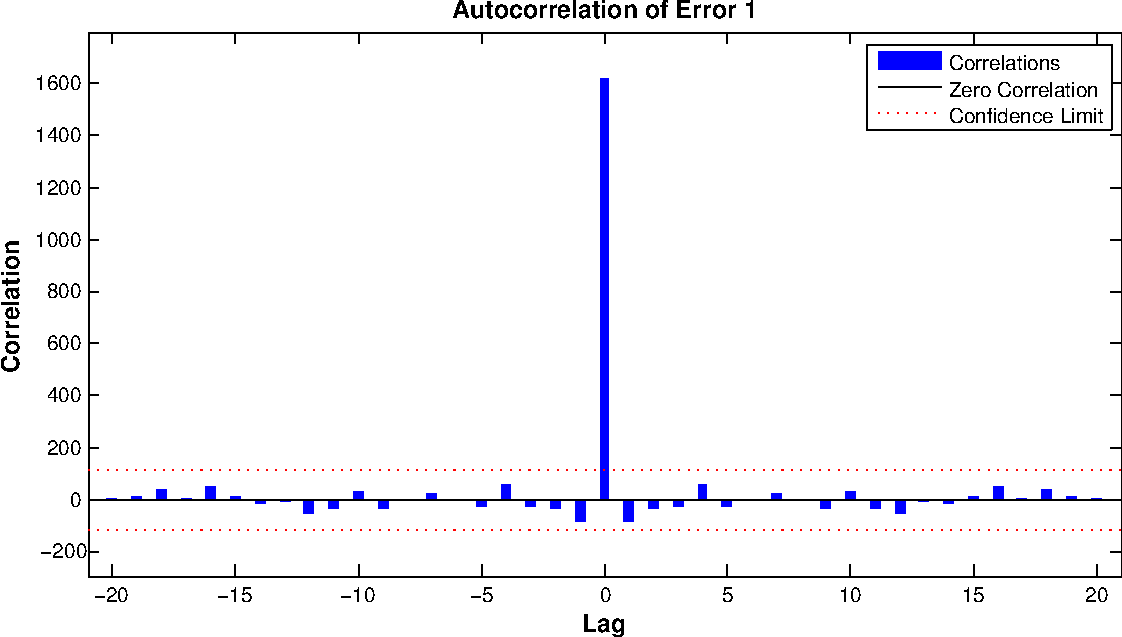
\includegraphics[scale=0.5]{images/timeseries/energia/autocorrelations.pdf}
  \caption{Autocorrelazione errore}
\end{figure}

\begin{figure}[htbp]
  \centering
  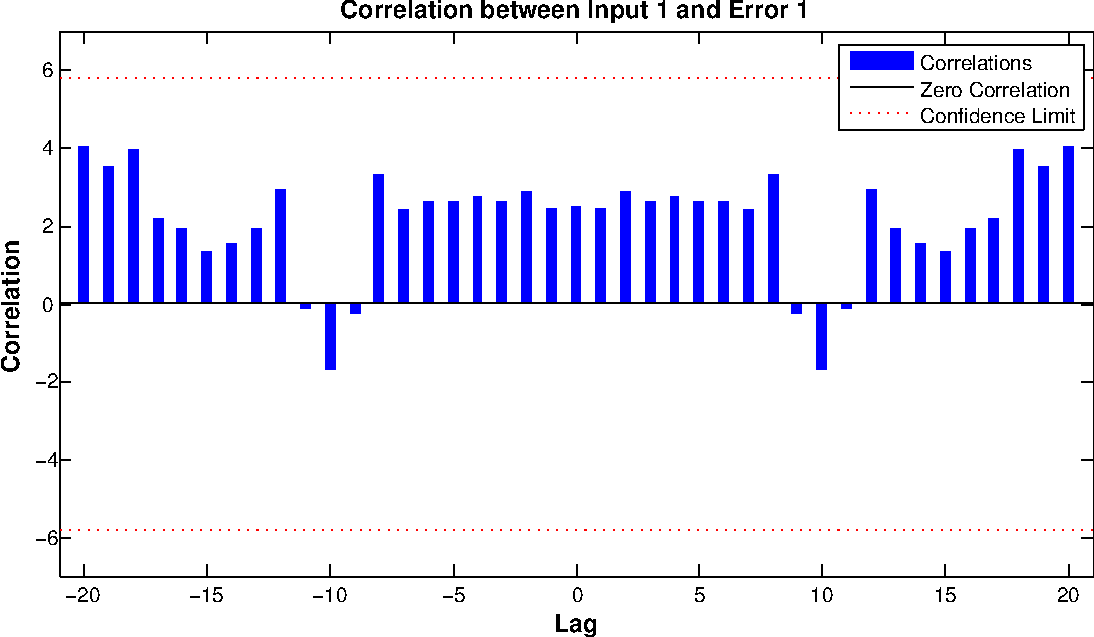
\includegraphics[scale=0.5]{images/timeseries/energia/correlations.pdf}
  \caption{Correlazione tra input e output}
\end{figure}


\paragraph{Luce interna}

\begin{figure}[htbp]
  \centering
  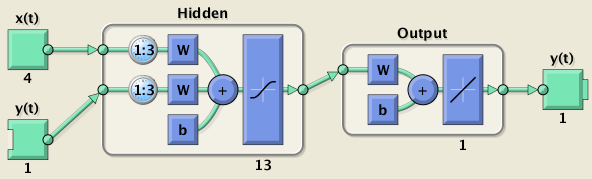
\includegraphics[scale=0.5]{images/timeseries/inlight/net.png}
  \caption{Rete usata}
\end{figure}

\begin{figure}[htbp]
  \centering
  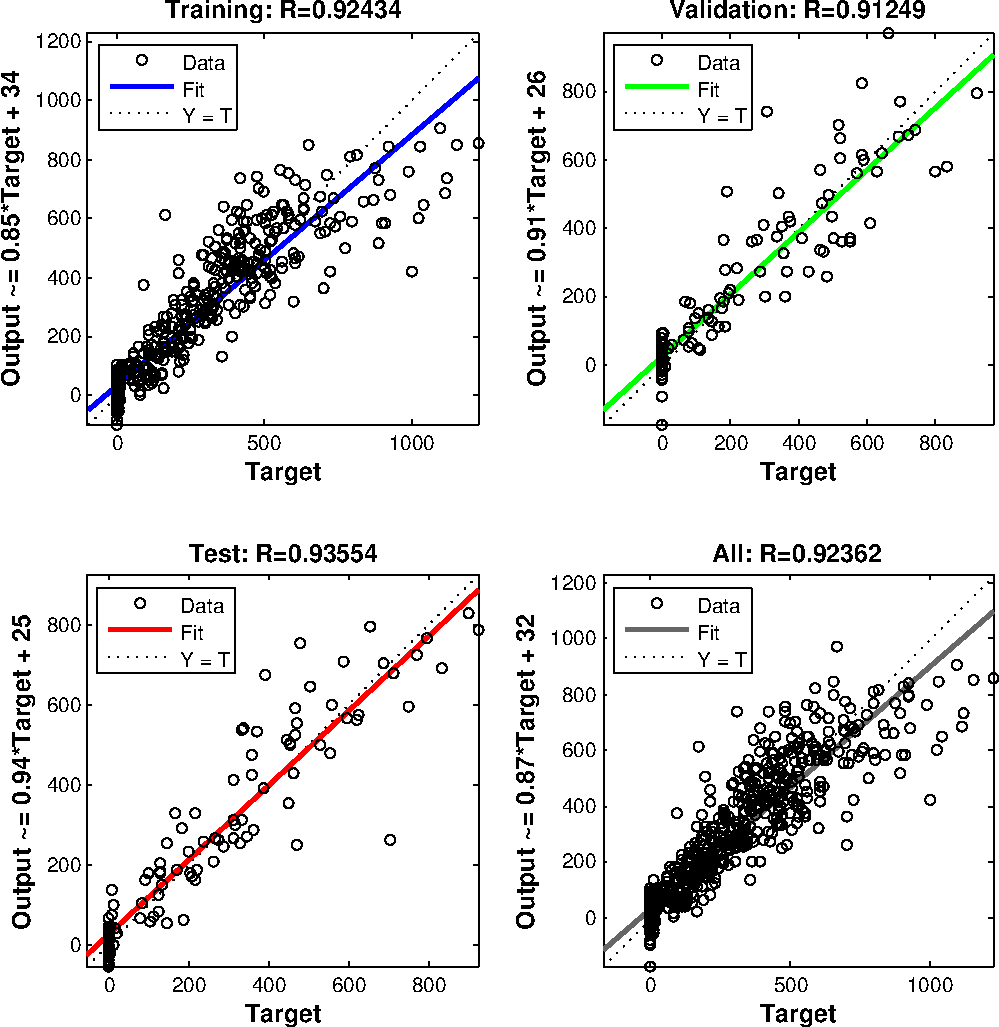
\includegraphics[scale=0.5]{images/timeseries/inlight/regressions.pdf}
  \caption{Retta di regressione}
\end{figure}

\begin{figure}[htbp]
  \centering
  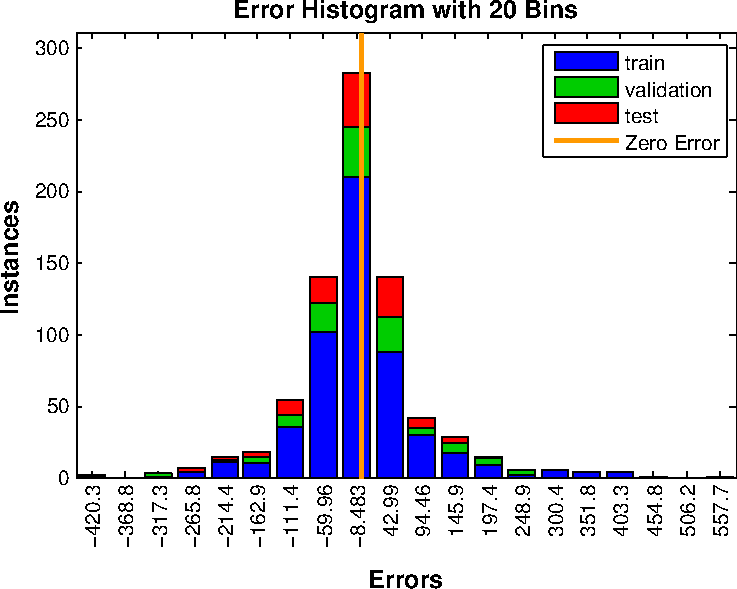
\includegraphics[scale=0.5]{images/timeseries/inlight/histogram.pdf}
  \caption{Istrogramma degli errori}
\end{figure}

\begin{figure}[htbp]
  \centering
  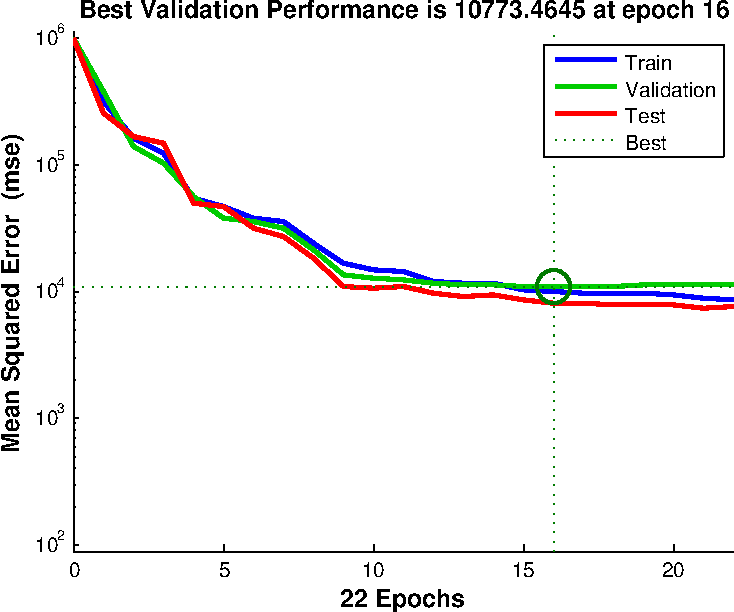
\includegraphics[scale=0.5]{images/timeseries/inlight/performances.pdf}
  \caption{Performance}
\end{figure}

\begin{figure}[htbp]
  \centering
  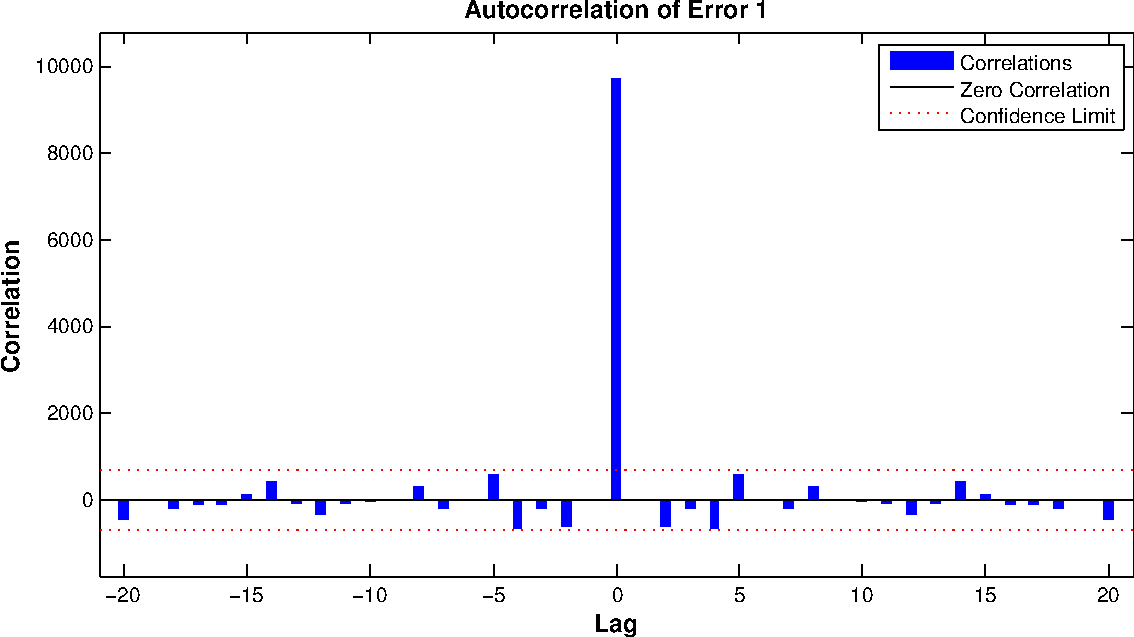
\includegraphics[scale=0.5]{images/timeseries/inlight/autocorrelations.pdf}
  \caption{Autocorrelazione errore}
\end{figure}

\begin{figure}[htbp]
  \centering
  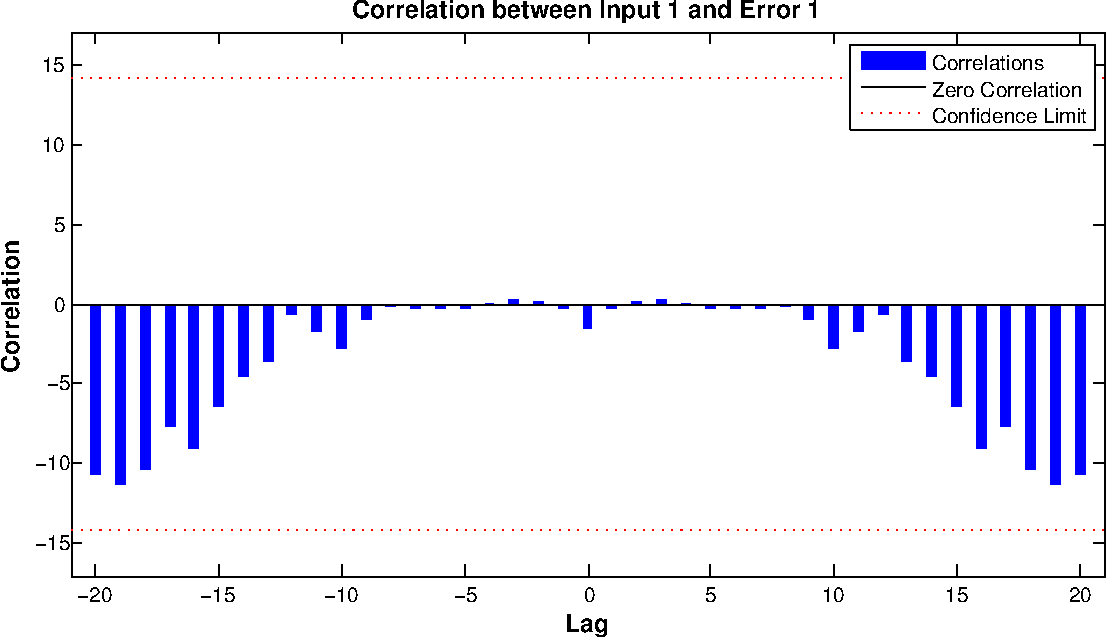
\includegraphics[scale=0.5]{images/timeseries/inlight/correlations.pdf}
  \caption{Correlazione tra input e output}
\end{figure}

\clearpage
